\documentclass[12pt]{article}
\usepackage{authblk}
\usepackage[utf8]{inputenc}
\usepackage[english]{babel}
\usepackage{graphicx}
\usepackage{calligra}
\usepackage{gensymb}
\usepackage{float}
\usepackage{siunitx}
\usepackage{amsmath}
\usepackage{grffile}
\usepackage[mathscr]{euscript}
\usepackage{multicol}
\usepackage[document]{ragged2e}
\usepackage[margin=1.0in]{geometry}
\usepackage{verbatim}
\setlength{\parskip}{0.25em}
\renewcommand{\baselinestretch}{0.25}
%%%%%%%%%%%%%%%%%%%%%%%%% Document Info
\title{The Raman Spectrum of Titanium Dioxide and Sulfur With a 785 nm Laser}
\author{Taylor Larrechea, Edward McClain}
\affil{Colorado Mesa University}
\affil{Department of Physical and Environmental Sciences}
\date{March 4, 2019}
\begin{document}
\maketitle
%%%%%%%%%%%%%%%%%%%%%%%%% Abstract
\begin{abstract}
\paragraph{}
\setlength{\parskip}{1em}
Stokes and anti-Stokes intensities were reported along with the relative wavenumbers for the Titanium dioxide sample as well as the Sulfur sample. The anti-Stokes and Stokes lines were found to be close to the same relative wavenumbers as one another regardless of what side of the spectrum that was being observed. The ratios of anti-Stokes to Stokes intensities were compared for both Titanium dioxide and Sulfur.
\end{abstract}
%%%%%%%%%%%%%%%%%%%%%%%%% Introduction
\section{Introduction}
\begin{multicols}{2}
\paragraph{}
\setlength{\parskip}{1em}
Raman Scattering is the scattering of photons via molecules resulting in excitation of vibrating modes [6]. There are two distinct areas (Ranges of relative wavenumbers) where this scattering effect can be observed. For this articles sake we will refer to the locations of these Raman Peaks, which are the locations of extremely high intensity, as both anti-Stokes and Stokes lines. The Stokes lines are lines of observed high intensity where the emitted photon has less energy, where as the anti-Stokes lines are lines of observed high intensity where the emitted photon has more energy after scattering into the material [6]. The Stokes and anti-Stokes lines were both named after George Stokes who first observed this scattering effect in 1852 [6]. 
\paragraph{}
\setlength{\parskip}{1em}
In this experiment the primary sample that is being observed is Titanium dioxide (TiO2). Titanium dioxide is a chalky white powder that is primarily used in cosmetics, toothpaste, adhesives, plastics, other consumer products, and the most applicable to this study, sunscreen [2]. Essentially, there are different kinds of Titanium dioxide. The first type is referred to as "Pigment-grade" Titanium dioxide. Pigment-grade Titanium dioxide is used primarily in items such as paints and coatings, plastics and adhesives, rubber, cosmetics, and paper products [2]. The other type of Titanium dioxide is called "Nanoscale Titanium dioxide". Nanoscale Titanium dioxide is used in primarily sunscreen and catalysts [2]. The reason why Titanium dioxide is used in sunscreen is because the particle size is extremely small, and this extremely small particle does not reflect visible light but rather absorbs UV light [2]. This phenomena of Nanoscale Titanium dioxide absorbing UV light is what makes it so applicable and useful in sunscreen. This is also a driving factor into why Titanium dioxide was used as a sample in this experiment. 
\end{multicols}
%%%%%%%%%%%%%%%%%%%%%%%%% Experimental
\section{Experimental}
\begin{multicols}{2}
\paragraph{}
\setlength{\parskip}{1em}
The equipment used in this experiment consisted of mirrors, beam splitters, stands to hold these objects, a 90 mW laser, and one Acton Spectropro SP-2300 spectrometer for analyzing the samples. The software that was used to observe the Raman Scattering in this experiment was called Light Field. The laser from the 90 mW source is directed to the Titanium dioxide sample that is suspended via a tray. After the laser contacts the sample that is being suspended, it is redirected to the spectrometer to be analyzed with the aide of Light Field. 
\paragraph{}
\setlength{\parskip}{1em}
The first step in collecting the data in this experiment once all the equipment was setup was to start up Light Field. Then all the settings had to be calibrated, including binning the data, making sure it outputs to the correct folder and in the right format, as well as setting the wavelength for the laser. After the experiment was setup and the software was initialized, the data could begin to be collected.
\end{multicols}
%%%%%%%%%%%%%%%%%%%%%%%%% Data and Results
\section{Data and Results}
\begin{multicols}{2}
\paragraph{}
\setlength{\parskip}{1em}
As previously stated, the exposure times that were used in this experiment were two, three, and four seconds. Since the data was readily accessible for multiple runs, there are a total of two graphs for each exposure time. One graph depicts the Stokes Lines and the other depicts the anti-Stokes Lines. Figure 1 shows the data points for the anti-Stokes lines of Titanium dioxide in a two second interval.
%%%%%%%%%%%%%%%%%%%%%%%%% Figure 1
\begin{center}
    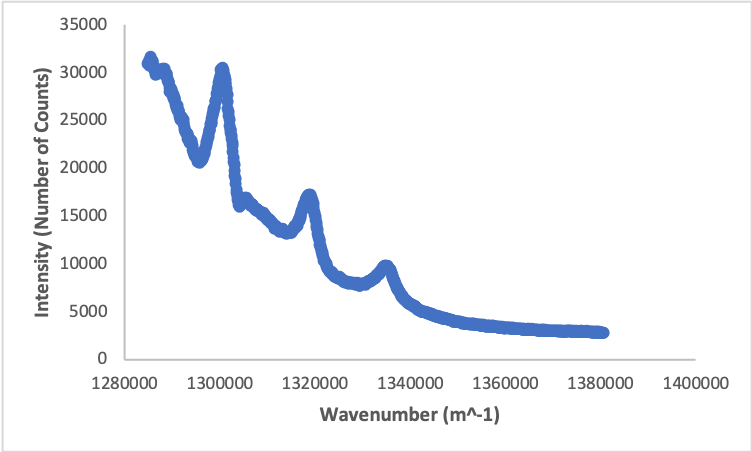
\includegraphics[width=7cm, height=4cm]{PHYS 331 RS TiO2 Antistokes Wavnumber (2 Sec).png}
    \caption{\textbf{\small{Figure 1:}} \small{Anti-Stokes Intensities of TiO2 at 2 Second Exposure. The first peak that occurred which is around 1300000 $m^-1$ can be neglected due to errors in the instruments of the experiment.}}
\end{center}
%%%%%%%%%%%%%%%%%%%%%%%%% Table 1
\begin{tabular}{|c|c|}
    \hline \textbf{\small Wavenumber (m$^{-1}$)} & \textbf{\small Intensity (Counts)} \\ \hline
    1.33458$\cdot10^6$ & 14,316 \\ \hline
    1.31874$\cdot10^6$ & 17,198 \\ \hline
    1.30039$\cdot10^6$ & 32,207 \\ \hline
\end{tabular}
\centerline{\tiny{\textbf{Table 1:}} \tiny{Anti-Stokes Intensities of TiO2 at 2 Second Exposure.}}
\newline
Figure 1 and Table 1 depict the results for the two second run of the anti-Stokes intensities. The intensities found in Table 1 were calculated with the use of a computer program called Fityk. To calculate the intensities of the peaks, Fityk calculated the area under the curve for each individual peak. The wavenumber on the other hand was able to be calculated with first finding the wavelength of the peak with excel, and then converting it to a wavenumber. Figure 2 shows the plot of data for the Stokes intensities of Titanium dioxide at the two second exposure.
%%%%%%%%%%%%%%%%%%%%%%%%% Figure 2
\begin{center}
    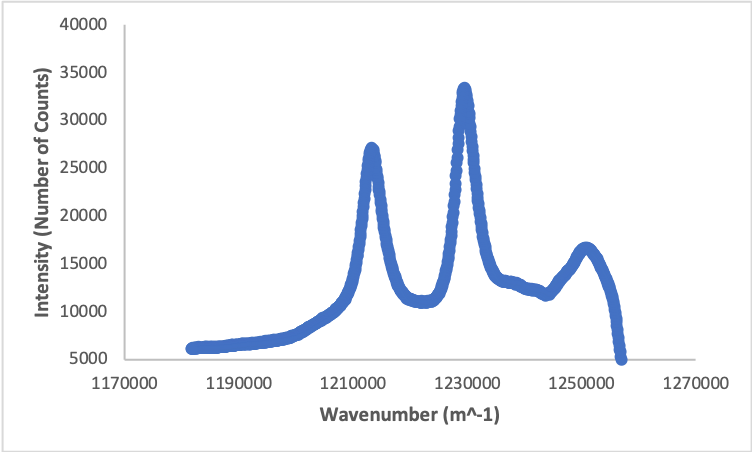
\includegraphics[width=7cm, height=4cm]{PHYS 331 RS TiO2 Stokes Wavnumber (2 Sec).png}
    \caption{\textbf{\small{Figure 2:}} \small{Stokes Intensities of TiO2 at 2 Second Exposure.}}
\end{center}
Figure 2 shows the Stokes intensities of TiO2 at three different wavenumbers. It should be noted that the relative wavenumbers are close to those found in the anti-Stokes plot in Figure 1. To better represent the Stokes intensities for TiO2 at the two second exposure Table 2 is constructed.
\newline
%%%%%%%%%%%%%%%%%%%%%%%%% Table 2
\begin{tabular}{|c|c|}
    \hline \textbf{Wavenumber (m$^{-1}$)} & \textbf{Intensity (Counts)} \\ \hline
    1.25047$\cdot10^6$ & 2,500 \\ \hline
    1.22971$\cdot10^6$ & 7,000 \\ \hline
    1.21344$\cdot10^6$ & 14,000 \\ \hline
\end{tabular}
\centerline{\tiny{\textbf{Table 2:}} \tiny{Stokes Intensities of TiO2 at 2 Second Exposure.}}
\newline
The intensities in Table 2 were calculated with a PsuedovoigtA tool in Fityk where as the intensities in Table 1 were calculated with a GaussianA tool. The choices of tools depended primarily on the shape of the peaks. In Figure 2, the peaks tend to be symmetric except for the last peak found around 1250000 m$^-1$. Because of this odd shape of the last peak, the PsuedovoigtA tool had to be used instead of the GaussianA tool. The two second interval has now been covered, the three second interval plot for the anti-Stokes intensities of Titanium dioxide can be seen in Figure 3.
%%%%%%%%%%%%%%%%%%%%%%%%% Figure 3
\begin{center}
    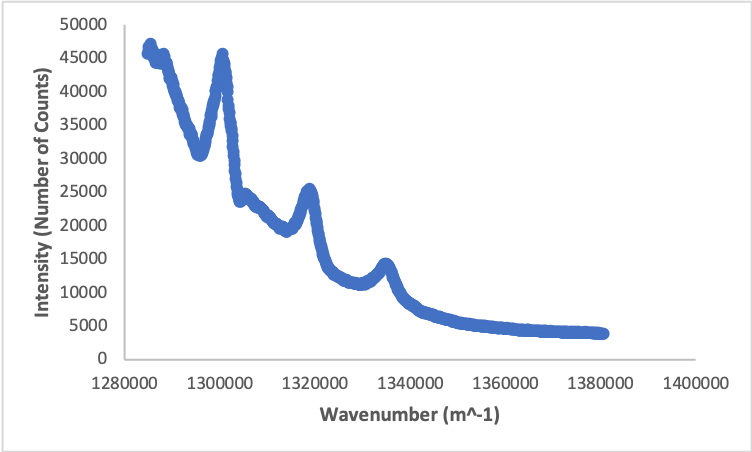
\includegraphics[width=7cm, height=4cm]{PHYS 331 RS TiO2 Antistokes Wavnumber (3 Sec).png}
    \caption{\textbf{\small{Figure 3:}} \small{Anti-Stokes Intensities of TiO2 at 3 Second Exposure. The same first peak can be neglected.}}
\end{center}
The intensities seen Figure 1 and Figure 3 are the biggest differences between the two time intervals. It should be expected that the intensity of the peaks will increase as the exposure time goes up because of the CCD component of the spectrometer having more time to collect data. These new intensities can be seen precisely in Table 3 below.
\newline
%%%%%%%%%%%%%%%%%%%%%%%%% Table 3
\begin{tabular}{|c|c|}
    \hline \textbf{Wavenumber (m$^{-1}$)} & \textbf{Intensity (Counts)} \\ \hline
    1.33494$\cdot10^6$ & 17,858 \\ \hline
    1.31857$\cdot10^6$ & 25,665 \\ \hline
    1.30039$\cdot10^6$ & 45,957 \\ \hline
\end{tabular}
\centerline{\tiny\textbf{{Table 3:}} \tiny{Anti-Stokes Intensities of TiO2 at 3 Second Exposure.}}
\newline
Brief inspection of these new intensities in Table 3 show that they increased relative to the intensities found in Table 1. The relative wavenumbers in Table 3 deviate from those found in Table 1 but this is not a vital component of the data. Although the relative wavenumber is important to report, the ratio of the anti-Stokes to Stokes intensities is the more important of the two. The same trend of higher reported intensities should be seen for the Stokes intensities in Figure 4 below.
%%%%%%%%%%%%%%%%%%%%%%%%% Figure 4
\begin{center}
    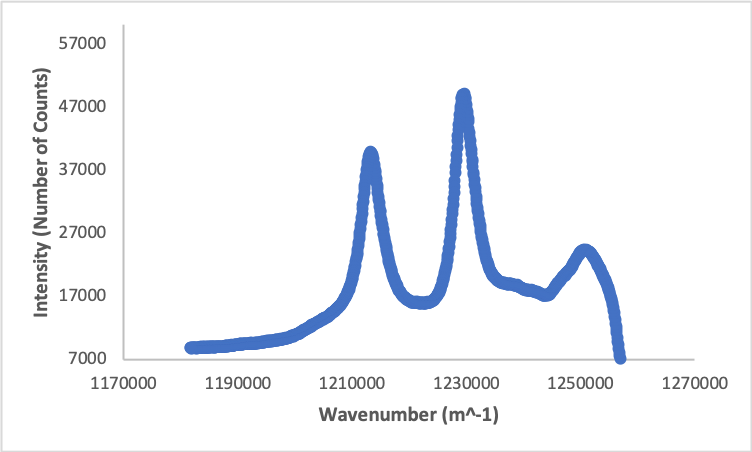
\includegraphics[width=7cm, height=4cm]{PHYS 331 RS TiO2 Stokes Wavnumber (3 Sec).png}
    \caption{\textbf{\small{Figure 4:}} \small{Stokes Intensities of TiO2 at 3 Second Exposure.}}
\end{center}
The intensities in Figure 4 have increased relative to those seen in Figure 2. To accurately depict this increase, Table 4 is constructed.
\newline
%%%%%%%%%%%%%%%%%%%%%%%%% Table 4
\begin{tabular}{|c|c|}
    \hline \textbf{Wavenumber (m$^{-1}$)} & \textbf{Intensity (Counts)} \\ \hline
    1.25078$\cdot10^6$ & 40,223 \\ \hline
    1.22971$\cdot10^6$ & 99,769 \\ \hline
    1.21344$\cdot10^6$ & 76,992 \\ \hline
\end{tabular}
\centerline{\tiny\textbf{{Table 4:}} \tiny{Stokes Intensities of TiO2 at 3 Second Exposure.}}
\newline
Figures 1 and 3 show anti-Stokes intensities of Titanium dioxide that are found at the same or close to the same wavenumber. The same can be said for Figures 2 and 4 where the only difference is that these intensities are the Stokes intensities of Titanium dioxide. As the exposure time increases, the current pattern shows that the intensities, regardless if it is the anti-Stokes or Stokes, are also increasing. The anti-Stokes intensities of Titanium dioxide with an exposure time of four seconds can be seen in Figure 5 below.
%%%%%%%%%%%%%%%%%%%%%%%%% Figure 5
\begin{center}
    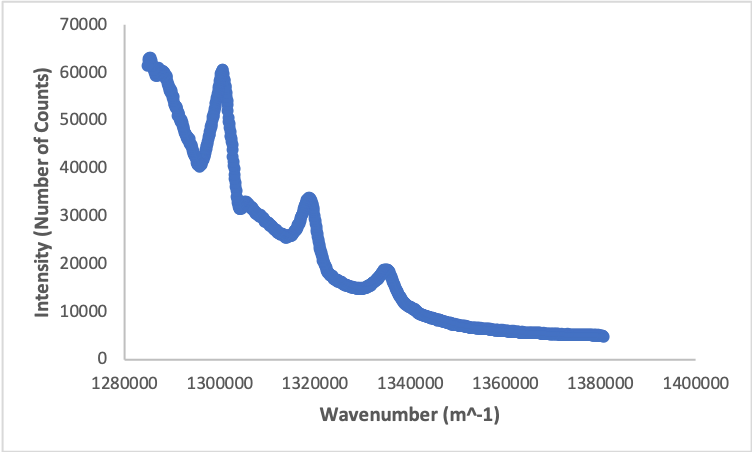
\includegraphics[width=7cm, height=4cm]{PHYS 331 RS TiO2 Antistokes Wavnumber (4 Sec).png}
    \caption{\textbf{\small{Figure 5:}} \small{Anti-Stokes Intensities of TiO2 at 4 Second Exposure. The first peak again can be neglected.}}
\end{center}
We once again see patterns for the anti-Stokes of Titanium dioxide that are consistent with those of the previous exposure times. To see the difference in anti-Stokes intensities, Table 5 is constructed.
\newline
%%%%%%%%%%%%%%%%%%%%%%%%% Table 5
\begin{tabular}{|c|c|}
    \hline \textbf{Wavenumber (m$^{-1}$)} & \textbf{Intensity (Counts)} \\ \hline
    1.33476$\cdot10^6$ & 16,548 \\ \hline
    1.31847$\cdot10^6$ & 32,530 \\ \hline
    1.30022$\cdot10^6$ & 67,916 \\ \hline
\end{tabular}
\centerline{\tiny\textbf{{Table 5:}} \tiny{Anti-Stokes Intensities of TiO2 at 4 Second Exposure.}}
\newline
Table 5 shows that the intensity of these peaks are continuing to increase. The only exception to this is the first peak which ended up being consequent of an error within the equipment of the experiment. The other two peaks ($1.31847\cdot10^6$ and $1.30022\cdot10^6$) both have intensities that increased relative to the previous exposure times. Figure 6 shows the Stokes intensities of Titanium dioxide at a four second exposure time.
%%%%%%%%%%%%%%%%%%%%%%%%% Figure 6
\begin{center}
    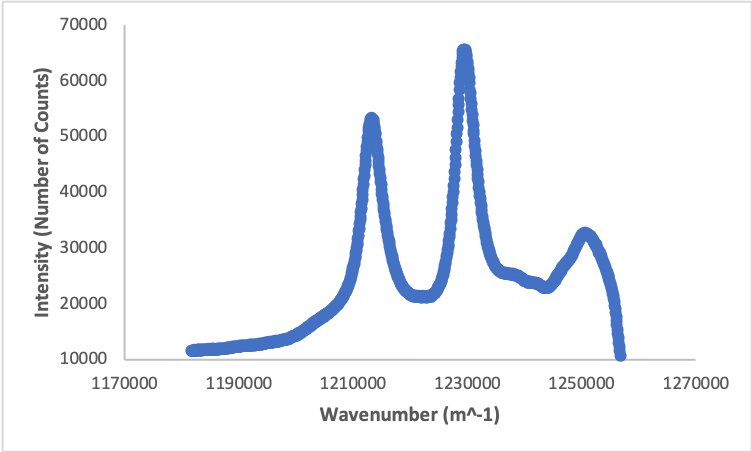
\includegraphics[width=7cm, height=4cm]{PHYS 331 RS TiO2 Stokes Wavnumber (4 Sec).png}
    \caption{\textbf{\small{Figure 6:}} \small{Stokes Intensities of TiO2 at 4 Second Exposure.}}
\end{center}
The wavenumbers at where these peaks occur are consistent with those observed in Figure 2 and Figure 4. The intensity differences can be seen in Table 6 below.
\newline
%%%%%%%%%%%%%%%%%%%%%%%%% Table 6
\begin{tabular}{|c|c|}
    \hline \textbf{Wavenumber (m$^{-1}$)} & \textbf{Intensity (Counts)} \\ \hline
    1.25078$\cdot10^6$ & 51,558 \\ \hline
    1.22971$\cdot10^6$ & 128,282 \\ \hline
    1.21344$\cdot10^6$ & 101,796 \\ \hline
\end{tabular}
\centerline{\tiny\textbf{{Table 6:}} \tiny{Stokes Intensities of TiO2 at 4 Second Exposure.}}
\newline
The intensities in Table 6 can be seen to have increased in comparison to both Table 2 and Table 4. We wish to run now the same procedure with Sulfur that we previously did with Titanium dioxide. Instead of doing three separate time exposures there is only one three second exposure for both the Stokes and anti-Stokes intensities of Sulfur that will be reported. Just as with the Titanium dioxide sample, Sulfur will have its own anti-Stokes to Stokes ratio for the intensity. Figure 7 below shows the anti-Stokes intensities for sulfur centered at -561 cm$^{-1}$.
%%%%%%%%%%%%%%%%%%%%%%%%% Figure 7
\begin{center}
    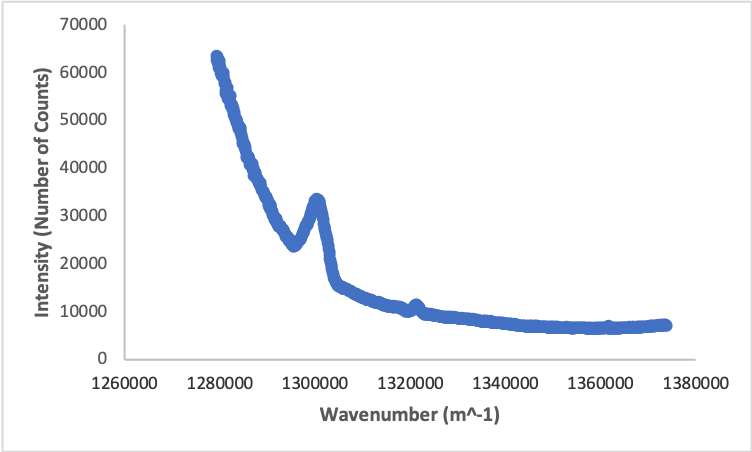
\includegraphics[width=7cm, height=4cm]{PHYS 331 RS S Anti-Stokes.png}
    \caption{\textbf{\small{Figure 7:}} \small{Stokes Intensities of Sulfur at 3 Second Exposure.}}
\end{center}
As with the Titanium dioxide sample, the intensities are the key measurement that we are after finding. Table 7 below shows the intensities for the two peaks for the Stokes side of Sulfur's Raman spectrum.
\newline
%%%%%%%%%%%%%%%%%%%%%%%%% Table 7
\begin{tabular}{|c|c|}
    \hline \textbf{Wavenumber (m$^{-1}$)} & \textbf{Intensity (Counts)} \\ \hline
    1.32135$\cdot10^6$ & 2,020 \\ \hline
    1.30039$\cdot10^6$ & 4,328 \\ \hline
\end{tabular}
\centerline{\tiny\textbf{{Table 7:}} \tiny{Stokes Intensities of Sulfur at 3 Second Exposure.}}
\newline
Contrary to the Titanium dioxide sample, the Sulfur sample only has two peaks with corresponding intensities that can be recorded. Table 7's purpose was to convey the intensities of these peaks at their corresponding wavenumber. Similar to the anti-Stokes intensities of Titanium dioxide, the GaussainA tool in the Fityk program was used to find the area of the two peaks under the curve as seen in Figure 7. Figure 8 shows the Stokes intensities of Sulfur centered at 561 cm$^{-1}$
%%%%%%%%%%%%%%%%%%%%%%%%% Figure 8
\begin{center}
    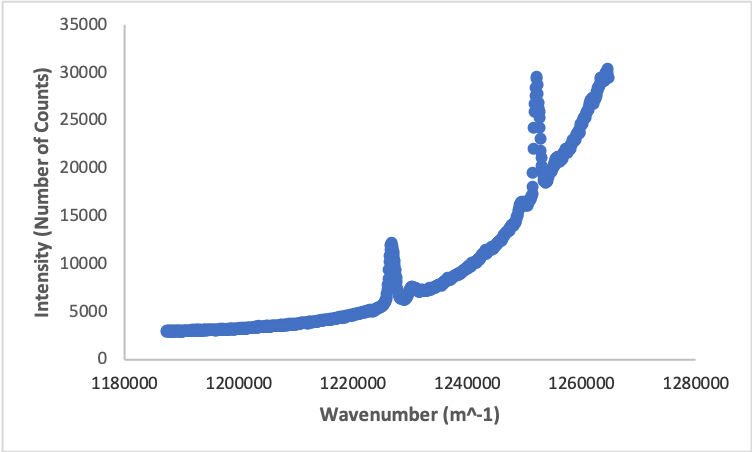
\includegraphics[width=7cm, height=4cm]{PHYS 331 RS S Stokes.png}
    \caption{\textbf{\small{Figure 8:}} \small{Stokes Intensities of Sulfur at 3 Second Exposure.}}
\end{center}
Similar to Figure 7, their are only two peaks to be found for the Stokes intensities of Sulfur centered at the specific wavenumber that we choose for this experiment. The intensities can be seen in Table 8 below.
\newline
%%%%%%%%%%%%%%%%%%%%%%%%% Table 8
\begin{tabular}{|c|c|}
    \hline \textbf{Wavenumber (m$^{-1}$)} & \textbf{Intensity (Counts)} \\ \hline
    1.25219$\cdot10^6$ & 8,826 \\ \hline
    1.22684$\cdot10^6$ & 5,772 \\ \hline
\end{tabular}
\centerline{\tiny\textbf{{Table 8:}} \tiny{Stokes Intensities of Sulfur at 3 Second Exposure.}}
\newline
Table 8 concludes the data collection of this experiment. The sulfur sample is observed to have again only two peaks where as the Titanium dioxide sample was showing three peaks at the $\pm$561 cm$^{-1}$ center wavenumbers. We can now move on to reporting the anti-Stokes to Stokes ratios of both Sulfur and Titanium dioxide.
\paragraph{}
\setlength{\parskip}{1em}
With the Titanium dioxide sample, there were three wavenumbers with corresponding intensities that were being reported for each time interval. The sulfur sample however had two wavenumbers that were found for the anti-Stokes and Stokes intensities. Because of this, one wavenumber was chosen in the Titanium dioxide sample for calculating the ratio where as both of the wavenumbers were used for the Sulfur sample. The wavenumber for the anti-Stokes intensity that will be used from each time interval for the Titanium dioxide sample is ($1.31874\cdot10^6$ m$^{-1}$), and the Stokes intensity is ($1.22971\cdot10^6$ m$^{-1}$). Taking an average and finding the standard deviation of the data, the anti-Stokes to Stokes ratio is
%%%%%%%%%%%%%%%%%%%%%%%%% Equation 1
\begin{equation}\label{1}
    \frac{AS}{S}=0.276153 \pm 0.030779
\end{equation}
where, "AS" is for anti-Stokes intensity of Titanium dioxide and, "S" is for the Stokes intensity of Titanium dioxide. The same procedure is ran with the data for Sulfur. The anti-Stokes to Stokes ratio for sulfur is
%%%%%%%%%%%%%%%%%%%%%%%%% Equation 2
\begin{equation}\label{2}
    \frac{AS}{S}=0.420167 \pm 0.070203.
\end{equation}
\end{multicols}
%%%%%%%%%%%%%%%%%%%%%%%%% Conclusion
\section{Conclusion}
\begin{multicols}{2}
\paragraph{}
\setlength{\parskip}{1em}
After running tests for both Titanium dioxide and Sulfur, the Sulfur sample was found to have a greater anti-Stokes to Stokes ratio than that of Titanium dioxide. As the tests were conducted, the intensities of the anti-Stokes and Stokes increased due to their being a longer capture time for the spectrometer, primarily the PIXIS CCD detector. More tests for the sulfur sample are required for more consistent data. A brief inspection between the intensities of the two peaks have two very different ratios for the anti-Stokes to Stokes intensities. To remedy this, more tests would need to be conducted for the sulfur sample to get more reliable data.
\end{multicols}
\newpage
%%%%%%%%%%%%%%%%%%%%%%%%% Bibliography
\begin{thebibliography}{8}
\bibitem{Alene Silva Melo Araújo}
Alene Silva Melo Araújo, Paula Ramalho Franca Flores, Victor Pinheiro Feitosa, Lídia Audrey Rocha Valadas, Diego Martins de Paula, Nicole de Mello Fiallos, Igor Ribeiro Rola, José Antero Soares Rola, Ana Cristina de Mello Fiallos. Micro-Raman Spectroscopy, Colour Stability, Roughness and Mass Variation of Removable Partial Dentures After Cleansing With White Wine Vinegar. Peer Reviewed. Fortaleza: Journal of Young Pharmacists, 2018.
\bibitem{Chemical Safety Facts}
Facts, Chemical Safey. Chemical Safety Facts. 1 March 2019. March 2019. <https://www.chemicalsafetyfacts.org/titanium-dioxide/>.
\bibitem{Gaoxiang MeiID}
Gaoxiang MeiID, Natalia Mamaeva, Srividya Ganapathy , Peng Wang , Willem J. DeGrip2, Kenneth J. RothschildI. Raman Spectroscopy of a Near Infrared Absorbing Proteorhodopsin: Similarities to the Bacteriorhodopsin O Photointermediate. Peer Reviewed. Boston: PLOS ONE, 2018.
\bibitem{Hiroaki ItoID}
Hiroaki ItoID, Naoyuki Uragami, Tomokazu Miyazaki, Noboru Yokoyama, Haruhiro Inoue. Raman Spectroscopic Evaluation of Human Serum Using Metal Plate and 785- nm and 1064- nm Excitation Lasers. Peer Reviewed. Koto: PLOS ONE, 2018.
\bibitem{Patrycja Garbacz}
Patrycja Garbacz, Marek Wesolowski. DSC, FTIR and Raman Spectroscopy Coupled with Multivariate Analysis in a Study of Co-Crystals of Pharmaceutical Interest. Peer Reviewed. Gdansk: MDPI, 2018.
\bibitem{Wikipedia Raman Scattering}
Wikipedia. Wikipedia. 31 January 2019. 16 February 2019. <https://en.Wikipedia.org/wiki/Raman$_$scattering>.
\bibitem{Yong Zhang}
Yong Zhang, Jingjing Xu, Yuezhou Yu, Wenhao Shang, Anpei Ye. Anti-Cancer Drug Sensitivity Assay with Quantitative Heterogeneity Testing Using Single-Cell Raman Spectroscopy. Peer Reviewed. Beijing: MDPI, 2018
\bibitem{Zheng-Yong Zhang}
Zheng-Yong Zhang, Dong-Dong Gui, Min Sha, Jun Liu, Hai-Yan Wang. Raman Chemical Feature Extraction for Quality Control of Dairy Products. Peer Reviewed. Zhejiang: American Dairy Science Association, 2019.
\end{thebibliography}


\end{document}
